\documentclass{standalone}

%\usepackage{amsmath}
\usepackage{tikz}
\usepackage[helvet]{sfmath}

\begin{document}

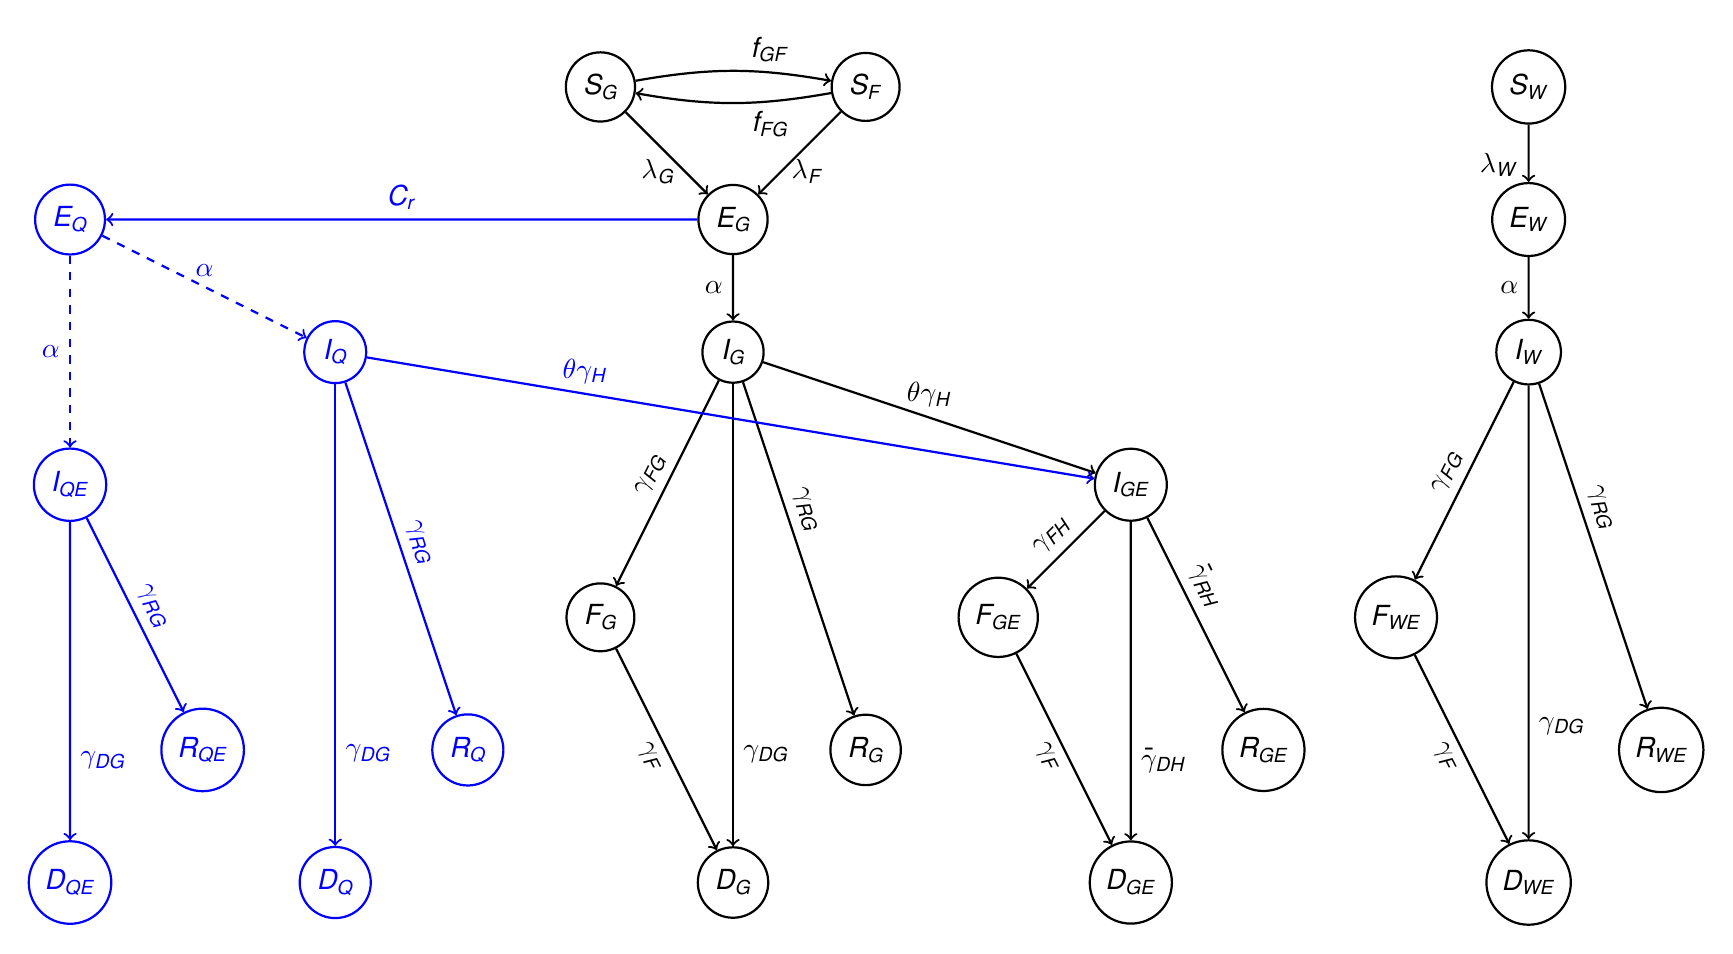
\begin{tikzpicture}[
  thick,
  scale = 0.842,
  compartment/.style = {circle, draw,
    minimum width = {width("$R_W$") + 2pt}}
  ]

  % Nodes
  \node at ( 0  , 14) [compartment, name = S_G] {$S_G$};
  \node at ( 4  , 14) [compartment, name = S_F] {$S_F$};
  \node at ( 14  , 14) [compartment, name = S_W] {$S_W$};


  \node at ( 2  ,  12) [compartment, name = E_G] {$E_G$};
  \node at ( 14  ,  12) [compartment, name = E_W] {$E_W$};
  \node at (-8, 12)  [compartment, name = E_Q,blue] {$E_Q$}; % contact
                                % tracing compartment


  \node at ( 2  ,  10) [compartment, name = I_G] {$I_G$};
  \node at ( -4  ,  10) [compartment, name = I_Q,blue] {$I_Q$};
  \node at (14,  10) [compartment, name = I_WE] {$I_{W}$};
  

  \node at (8 ,  8) [compartment, name = I_GE] {$I_{GE}$};
  \node at (-8,  8) [compartment, name = I_QE,blue] {$I_{QE}$};
  
  
  \node at (0  , 6) [compartment, name = F_G] {$F_G$};
  \node at (6 ,  6) [compartment, name = F_GE] {$F_{GE}$};
  \node at (12  ,6) [compartment, name = F_WE] {$F_{WE}$};
 
 

  \node at ( 4  ,  4) [compartment, name = R_G] {$R_G$};
  \node at (10,  4) [compartment, name = R_GE] {$R_{GE}$};
  \node at (16  , 4) [compartment, name = R_WE] {$R_{WE}$};
 \node at ( -2  ,  4) [compartment, name = R_Q,blue] {$R_Q$};
 \node at ( -6  ,  4) [compartment, name = R_QE,blue] {$R_{QE}$};


  \node at ( 2  ,  2) [compartment, name = D_G] {$D_G$};
  \node at ( 8,  2) [compartment, name = D_GE] {$D_{GE}$};
  \node at ( 14  ,2) [compartment, name = D_WE] {$D_{WE}$};
  \node at ( -4  ,  2) [compartment, name = D_Q, blue] {$D_Q$};
  \node at ( -8  ,  2) [compartment, name = D_QE, blue] {$D_{QE}$};
  




  % % Rates
   \draw [->] (S_G) to [out =   10, in = 170] node [above, pos = 0.7]
   {$f_{GF}$} (S_F);
   \draw [->] (S_F) to [out = -170, in = -10] node [below, pos = 0.3]
   {$f_{FG}$} (S_G);

  
  
   \draw [->] (S_G) to node [left , pos = 0.72] {$\lambda_G$} (E_G);
   \draw [->] (S_F) to node [right, pos = 0.72]      {$\lambda_F$} (E_G);
   \draw [->] (S_W) to node [left , pos = 0.7 ] {$\lambda_W$} (E_W);

   \draw [->] (E_G) to node [left] {$\alpha$} (I_G);
   \draw [->] (E_W) to node [left]   {$\alpha$} (I_WE);


   \draw [->] (I_G) to node [above] {$\theta \gamma_H $} (I_GE);
  

 
   \draw [->] (I_G) to node [sloped, above]    {$\gamma_{FG}$} (F_G);
   
   \draw [->] (I_GE) to node [sloped, above]    {$\gamma_{FH}$} (F_GE);
   \draw [->] (I_WE) to node [sloped, above]    {$\gamma_{FG}$}
   (F_WE);
   

   \draw [->] (I_G) to node [sloped, above, pos = 0.4]  {$\gamma_{RG}$} (R_G);
   \draw [->] (I_GE) to node [sloped, above, pos = 0.4]  {$\bar{\gamma}_{RH}$}       (R_GE);
   \draw [->] (I_WE) to node [sloped, above, pos = 0.4]  {${\gamma}_{RG}$}       (R_WE);

   \draw [->] (I_G) to node [right,pos = 0.8]  {${\gamma}_{DG}$} (D_G);
   \draw [->] (I_GE) to node [right,pos = 0.75] {$\bar{\gamma}_{DH}$}
   (D_GE);
   \draw [->] (I_WE) to node [right,pos = 0.75] {${\gamma}_{DG}$} (D_WE);
  
   \draw [->] (F_G) to node [sloped, below] {$\gamma_F$} (D_G);
   \draw [->] (F_GE) to node [sloped, below] {$\gamma_F$} (D_GE);
   \draw [->] (F_WE) to node [sloped, below] {$\gamma_F$} (D_WE);

% Contact tracing rates

\draw [->,blue] (E_G) to node [above] {$C_r$} (E_Q);

% if ebola center is full
\draw [->,blue] (I_Q) to node [above,pos=0.3] {$\theta \gamma_H$} (I_GE);
\draw [dashed,->,blue] (E_Q) to node [above] {$\alpha$} (I_Q);
%\draw [->,blue] (I_Q) to node [sloped,above] {$\gamma_{FG}$} (F_Q);
\draw [->,blue] (I_Q) to node [sloped,above] {$\gamma_{RG}$} (R_Q);
\draw [->,blue] (I_Q) to node [right,pos = 0.8] {$\gamma_{DG}$} (D_Q);
%\draw [->,blue] (F_Q) to node [sloped,below] {$\gamma_F$} (D_Q);

% if ebola center is not full
\draw [dashed,->,blue] (E_Q) to node [left] {$\alpha$} (I_QE);
%\draw [->,blue] (I_QE) to node [sloped,above] {$\gamma_{FG}$} (F_QE);
\draw [->,blue] (I_QE) to node [sloped,above] {$\gamma_{RG}$} (R_QE);
\draw [->,blue] (I_QE) to node [right,pos = 0.75] {$\gamma_{DG}$} (D_QE);
%\draw [->,blue] (F_QE) to node [sloped,below] {$\gamma_F$} (D_QE);


\end{tikzpicture}


\end{document}
